\input{../../main}

\begin{document}

\setphysstyle{ГЦФО 8}{Серия Ш-04}{05.10.2016}

\Large
\setcounter{notask}{12}

\task{ Куб из однородного материала плавает, погрузившись на глубину
  $h$ в жидкость. На какую глубину $H$ в этой же жидкости погрузится
  куб, имеющий вдвое б\textbf{о}льшую плотность и вдвое
  б\textbf{о}льшую длину ребра? }
% Максвелл-2016, 8 класс

\taskpic{ В цилиндрическом стакане находилось 4
  шарика. Экспериментатор аккуратно с помощью шприца добавлял в стакан
  жидкость и заносил в таблицу значения высоты уровня жидкости в
  стакане в зависимости от объёма добавленной жидкости. Известно, что
  в процессе эксперимента шарики не всплывали. По результатам
  измерений определите площадь сечения стакана и объём одного
  шарика. }
{
  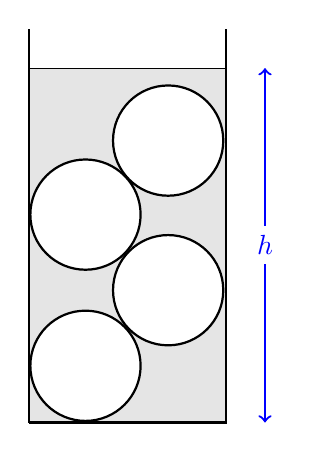
\begin{tikzpicture}
    \draw[fill=gray!20] (0,0) rectangle ++(2.5,4.5);
    \draw[thick] (0,0) -- ++(2.5,0) -- ++(0,5);
    \draw[thick] (0,0) -- ++(0,5);
    \draw[fill=white,thick] (0.72,0.72) circle (0.7cm);
    \draw[fill=white,thick] (1.77,1.68) circle (0.7cm);
    \draw[fill=white,thick] (0.72,2.64) circle (0.7cm);
    \draw[fill=white,thick] (1.77,3.58) circle (0.7cm);
    \draw[thick,blue,<->] (3,0) -- (3,4.5) node[midway,fill=white] {$h$}; 
  \end{tikzpicture}
}

\begin{table}[h]
  \centering
  \large
  \begin{tabular}{|c|c|c|c|c|c|c|c|c|c|c|c|c|c|}
    \hline
    $V,\unit{см}^3 $ & 0 & 50 & 100 & 150 & 200 & 250 & 300 & 350 & 400
    & 450 & 500 & 550 & 600\\
    \hline
    $h, \unit{см}$ & 0 & 1,2 & 2,7 & 4,1 & 5,3 & 7,0 & 9,0 & 10,5 &
                                                                     12,0
    & 13,0 & 14,0 & 15,0 & 16,0  \\
    \hline
  \end{tabular}
\end{table}
% Максвелл-2016, 8 класс

\taskpic{ В герметичном сосуде сверху находится жидкость с плотностью
  $\rho_0 = 800 \kgm$, отделённая лёгким подвижным поршнем от газа,
  находящегося внизу и имеющего давление $p=20\unit{кПа}$. В поршне
  есть круглое отверстие, в которое вставлен цилиндрический
  поплавок. В жидкость поплавок погружен на длину $h$, а в газ на
  длину $3h$. Площадь основания поплавка $S$. Поплавок может свободно
  скользить относительно поршня, а поршень относительно стенок сосуда.
  Жидкость нигде не подтекает. Какой должна быть плотность поплавка
  $\rho$, чтобы система могла оставаться в равновесии? Ускорение
  свободного падения $g = 10\mc$. }
{
  \begin{tikzpicture}
    \draw[thick] (0,0) rectangle ++(4,5);
    \draw[fill=gray!70] (0,3.3) rectangle ++(1.5,0.1);
    \draw[fill=gray!70] (4,3.3) rectangle ++(-1.5,0.1);
    \draw[fill=gray!20] (1.5,4) rectangle ++(1,-2.8);
    \draw[blue,thick,<->] (1.7,4) -- ++(0,-0.7) node[midway,right]
    {$h$}; 
    \draw[blue,thick,<->] (1.7,3.3) -- ++(0,-2.1) node[midway,right=-0.1cm]
    {$3h$};
    \draw (0.2,0) node[anchor = south west] {\normalsize газ};
    \draw (0.2,4.4) node[anchor = south west] {\normalsize жидкость};
    \draw (3.7,4.7) node {\normalsize $\rho_0$};
    \draw (3.7,0.3) node {\normalsize $p$}; 
  \end{tikzpicture}
}
% Максвелл-2014, 8 класс

\end{document}


%%% Local Variables: 
%%% mode: latex
%%% TeX-engine:xetex
%%% TeX-PDF-mode: t
%%% End:
